\documentclass[aspectratio=169]{beamer}

\usepackage{amsmath}
\usepackage{booktabs}
\usepackage{comment}
\usepackage{graphicx}
\usepackage{xcolor}

\IfFileExists{lato.sty}{
    \usepackage[default]{lato}
}{}

\definecolor{pgpblue}{RGB}{0,114,178}
\definecolor{pgpred}{RGB}{213,94,0}
\definecolor{pgpgreen}{RGB}{0,158,115}
\definecolor{pgpbackground}{RGB}{255,255,255}

\setbeamercolor{background canvas}{bg=pgpbackground}
\setbeamercolor{normal text}{fg=black,bg=pgpbackground}
\setbeamercolor{structure}{fg=pgpblue}
\setbeamercolor{frametitle}{fg=pgpblue,bg=pgpbackground}
\setbeamercolor{title}{fg=black}
\setbeamercolor{itemize item}{fg=pgpblue}
\setbeamercolor{itemize subitem}{fg=pgpblue}
\setbeamercolor{enumerate item}{fg=pgpblue}

\setbeamerfont{title}{series=\bfseries,size=\Large}
\setbeamerfont{frametitle}{series=\bfseries,size=\large}
\setbeamertemplate{navigation symbols}{}
\setbeamertemplate{footline}[frame number]
\setbeamertemplate{itemize items}[circle]
\setbeamertemplate{section in toc}[sections numbered]

\title{CEMAC Jobs Analytics}
\subtitle{Cameroon elasticities and WBES trade diagnostics}
\author{}
\date{\today}

\begin{document}

\begin{frame}[plain]
    \titlepage
\end{frame}

\begin{frame}{Roadmap}
    \tableofcontents
\end{frame}

\section{BDF Cleaning Results}

\begin{frame}{Data cleaning overview}
    \begin{itemize}
        \item The working panel is organized at the firm-year level, so duplicate handling changes both sample size and identification.
        \item Economic sector is based on the NACAM variable, which according to documentation its based on a Regional harmonized classifier linked to ISIC.
        \item The cleaning note isolates the two steps that most affect downstream interpretation: duplicate resolution and the NACAM-to-ISIC crosswalk.
    \end{itemize}
\end{frame}

\begin{frame}{Firm-Year Duplicate Cleaning}
    \footnotesize
    \begin{itemize}
        \item Working key: \texttt{firmid} $\times$ \texttt{fin\_yr}
        \item Perfect duplicates would be collapsed with original row order as the tie-breaker.
        \item Conflicting duplicate firm-years are fully removed from the cleaned analysis file, while we figure out the best approach for handling them.
    \end{itemize}

    \vspace{0.2cm}
    \centering
    \resizebox{0.76\textwidth}{!}{
        \begin{tabular}{lr}
                        &       Value\\
\midrule
Original observations&       9,325\\
Perfect duplicate firm-years&           0\\
Rows dropped from perfect duplicates&           0\\
Conflicting duplicate firm-years&         127\\
Rows dropped from conflicting duplicates&         257\\
Final cleaned observations&       9,068\\

        \end{tabular}
    }
\end{frame}
\begin{comment} 
    % Lets confirm this but I think that we are not using the ISIC codes for the elasticity analysis, so we can skip this slide if we want to save time.
    % We can also move it to the appendix if we want to keep it for reference but not spend time on it in the main presentation.
\begin{frame}{NACAM-to-ISIC Crosswalk}
    \small
    \begin{itemize}
        \item Observed legacy NACAM codes are audited directly from the Cameroon BDF file.
        \item Legacy branch labels are recovered from the INS RGE nomenclature document, while the mapping to \texttt{NACAM rev.1} and ISIC comes from the official \texttt{NACAM rev.1} passage tables.
        \item ISIC Rev.4 divisions are assigned only when the official mapping is one-to-one.
        \item Ambiguous branches remain flagged for manual review rather than being forced into a noisy division code.
        \item Since the NACAM is already based on the ISIC structure, the analysis file retains the original NACAM variable for elasticity estimation and reporting, while the ISIC variable is used for sectoral aggregation and cross-country comparisons.
    \end{itemize}

    \vspace{0.4cm}
    \centering
    \resizebox{0.75\textwidth}{!}{
        \begin{tabular}{lr}
                        &       Value\\
\midrule
Observed legacy NACAM codes covered&          37\\
Codes with exact ISIC Rev.4 division assignment&          17\\
Codes flagged for manual review&          20\\

        \end{tabular}
    }
\end{frame}
\end{comment}

\begin{frame}{Cleaning Takeaways}
    \begin{itemize}
        \item The cleaned panel resizes the sample from 9,325 to 9,068 observations after removing duplicate firm-years.
        \item There are 127 conflicting firm-years, accounting for 257 dropped obs. Those observations are excluded rather than resolved ad hoc.
        %\item The crosswalk covers 37 observed legacy NACAM codes, but only 17 map cleanly to a single ISIC Rev.4 division. 
        \item To avoid introducing unwanted noise we keep the analysis using NACAM classification and link it to ISIC aggregates when possible.
        %\item The remaining 20 codes are explicitly flagged for manual review, which keeps sector harmonization transparent before pooled industry comparisons.
    \end{itemize}
\end{frame}

\section{Cameroun Census data on firm counts, employment, and revenue}

\begin{frame}{Cameroun Census Context}
    \begin{itemize}
        \item The 2024 RGE census gives a whole-economy snapshot of establishments in Cameroon.
        \item Census activity labels are harmonized to the same NACAM sectors used in the administrative elasticity analysis.
        \item The next slides use headquarter-level data to show sector scale in firm counts, log employment, log annual revenue, and log revenue per worker.
        \item After this economy-wide view, the administrative tax panel focuses on formal firms observed over time, using the administrative data.
    \end{itemize}
\end{frame}

\begin{frame}{Census Firm Counts by Harmonized NACAM Sector}
    \centering
    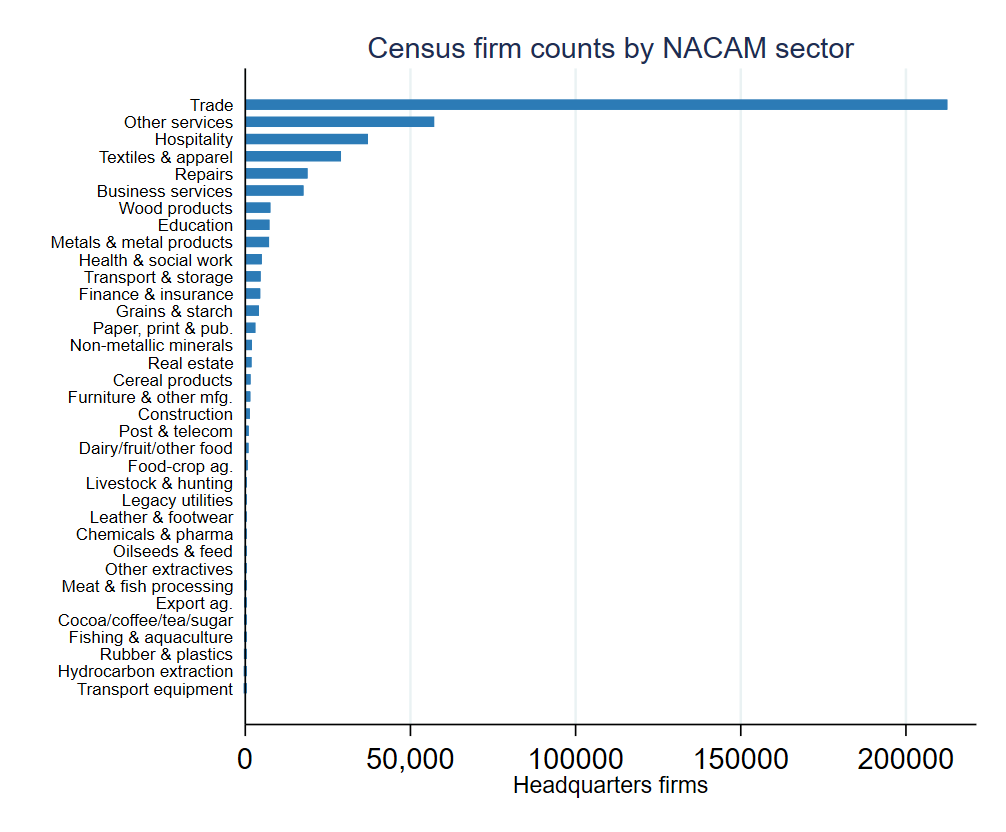
\includegraphics[width=\textwidth,height=0.76\textheight,keepaspectratio]{../output/figures/cmr_census_firm_count_by_nacam.png}
\end{frame}

\begin{frame}{Census Log Employment by Harmonized NACAM Sector}
    \centering
    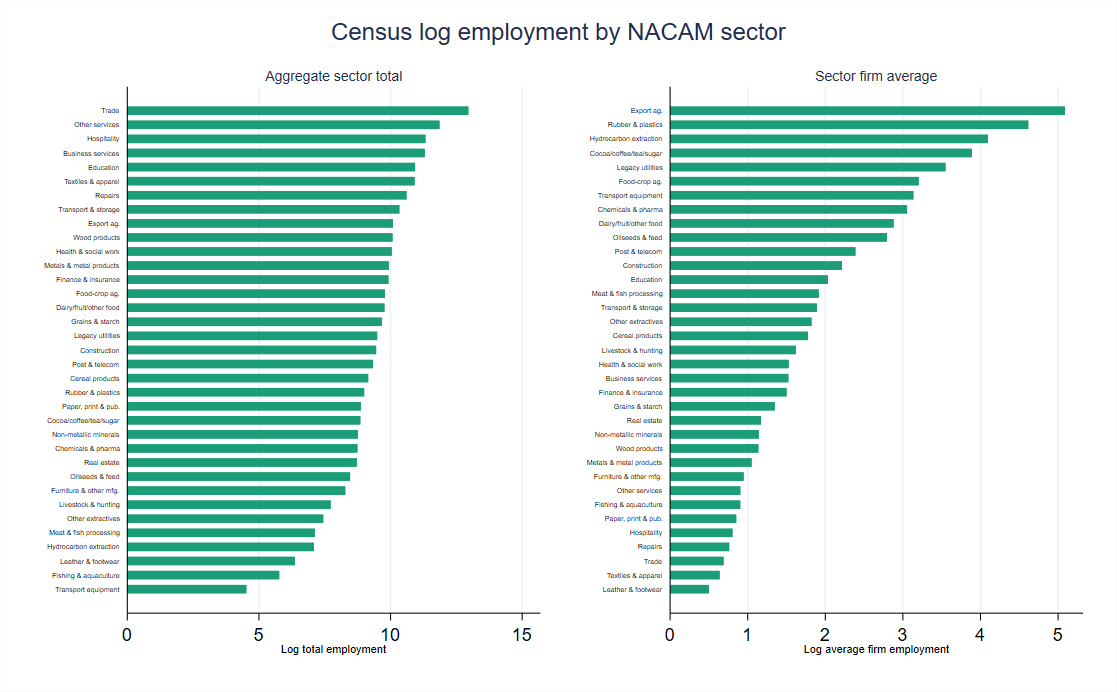
\includegraphics[width=\textwidth,height=0.76\textheight,keepaspectratio]{../output/figures/cmr_census_total_employment_by_nacam.png}
\end{frame}

\begin{frame}{Census Log Revenue by Harmonized NACAM Sector}
    \centering
    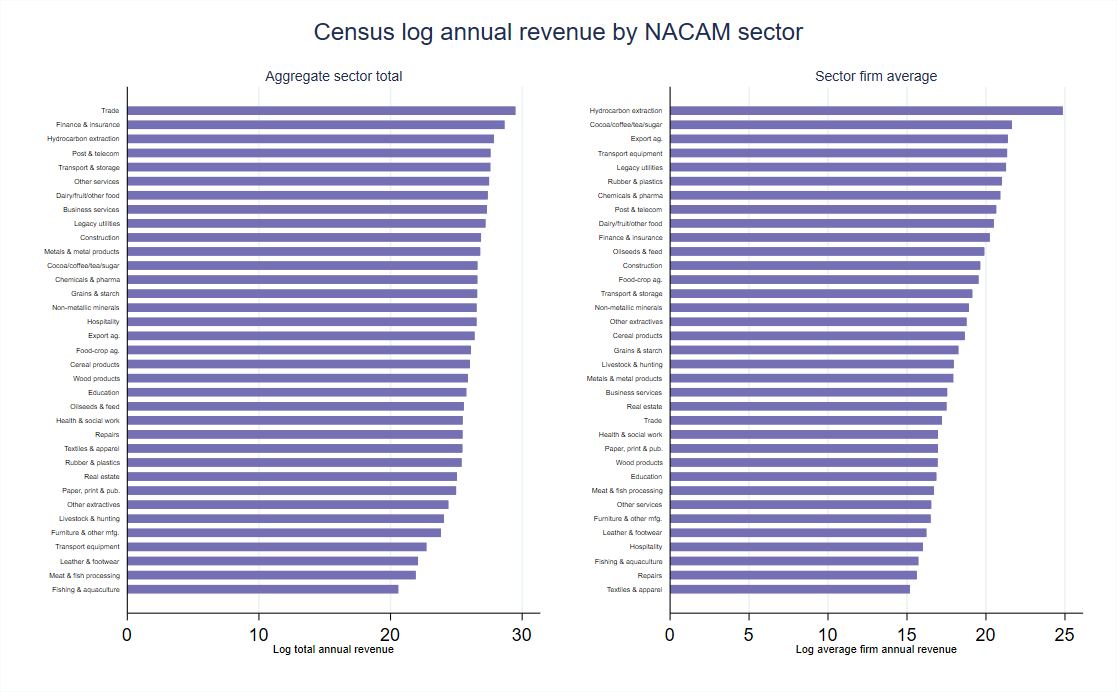
\includegraphics[width=\textwidth,height=0.76\textheight,keepaspectratio]{../output/figures/cmr_census_total_revenue_by_nacam.png}
\end{frame}

\begin{frame}{Census Log Revenue per Worker by Harmonized NACAM Sector}
    \centering
    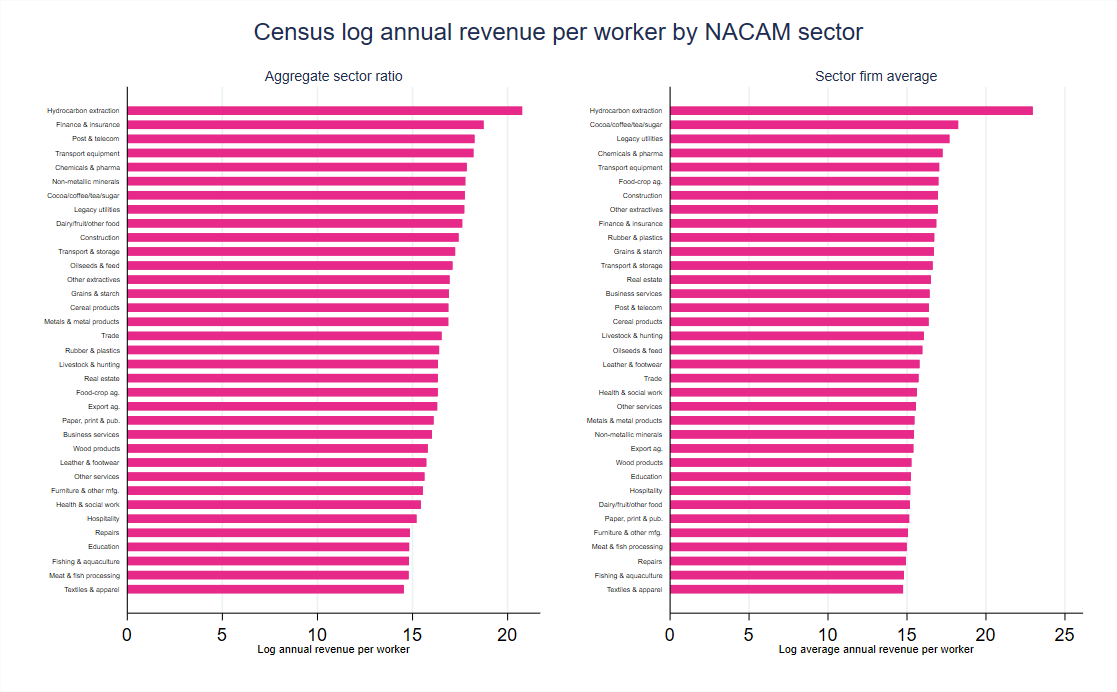
\includegraphics[width=\textwidth,height=0.76\textheight,keepaspectratio]{../output/figures/cmr_census_turnover_per_worker_by_nacam.png}
\end{frame}

\section{Cameroun Sectoral Elasticities}

\begin{frame}{Specification and Sample}
    \small
    \begin{equation}
        \ln(E_{it}) = \alpha_i + \delta_{st} + \sum_s \beta_s \left( \ln(X_{it}) \times D_{is} \right) + \varepsilon_{it}
    \end{equation}

    \begin{itemize}
        \item The unit of observation is a firm-year $(i,t)$.
        \item $E_{it}$ is employment for firm $i$ in year $t$.
        \item $X_{it}$ is either value added or total revenue, estimated in separate regressions.
        \item $D_{is}$ equals 1 if firm $i$ belongs to NACAM sector $s$, and 0 otherwise.
        \item Sector is treated as a firm characteristic, so each firm contributes to one NACAM interaction term.
        \item $\alpha_i$ are firm fixed effects and $\delta_{st}$ are sector-by-year effects.
        \item $\beta_s$ is the elasticity for firms in sector $s$, identified through the interaction between $\ln(X_{it})$ and the sector indicator $D_{is}$.
        \item Standard errors clustered at the firm level.
        \item Inclusion rule for reported sectors: at least 30 observations and 10 firms in both outcome samples.
    \end{itemize}
\end{frame}

\begin{frame}{Employment Distribution by Fiscal Year}
    \centering
    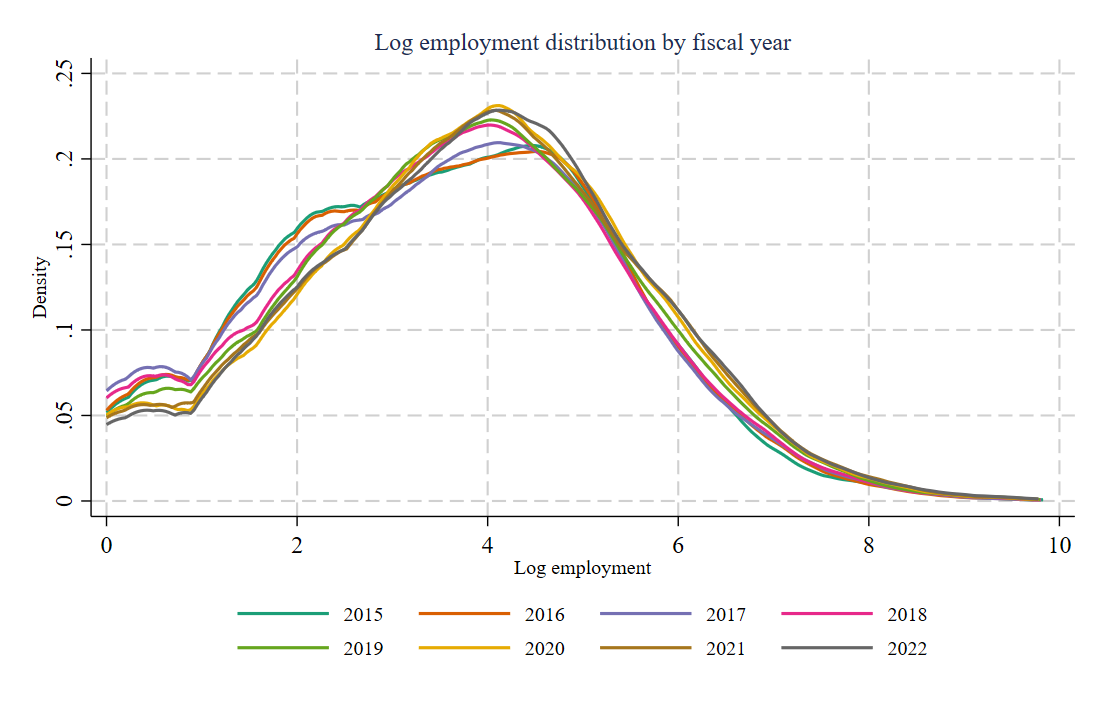
\includegraphics[width=\textwidth,height=0.76\textheight,keepaspectratio]{../output/figures/cmr_nacam_results_en_labels_ln_emp_density_by_year.png}
\end{frame}

\begin{frame}{Value-Added Elasticity Specification}
    \small
    \begin{equation}
        \ln(E_{it}) = \alpha_i + \delta_{st} + \sum_s \beta^{VA}_s \left( \ln(VA_{it}) \times D_{is} \right) + \varepsilon_{it}
    \end{equation}

    \begin{itemize}
        \item Estimates use the Cameroon administrative firm-year panel.
        \item Firm fixed effects absorb time-invariant firm differences.
        \item Sector-by-year effects absorb shocks common to a NACAM sector in a fiscal year.
        \item The plotted point for each sector is $\beta^{VA}_s$ with a firm-clustered 95 percent interval.
    \end{itemize}
\end{frame}

\begin{frame}{Value-Added Elasticities Across NACAM Sectors}
    \centering
    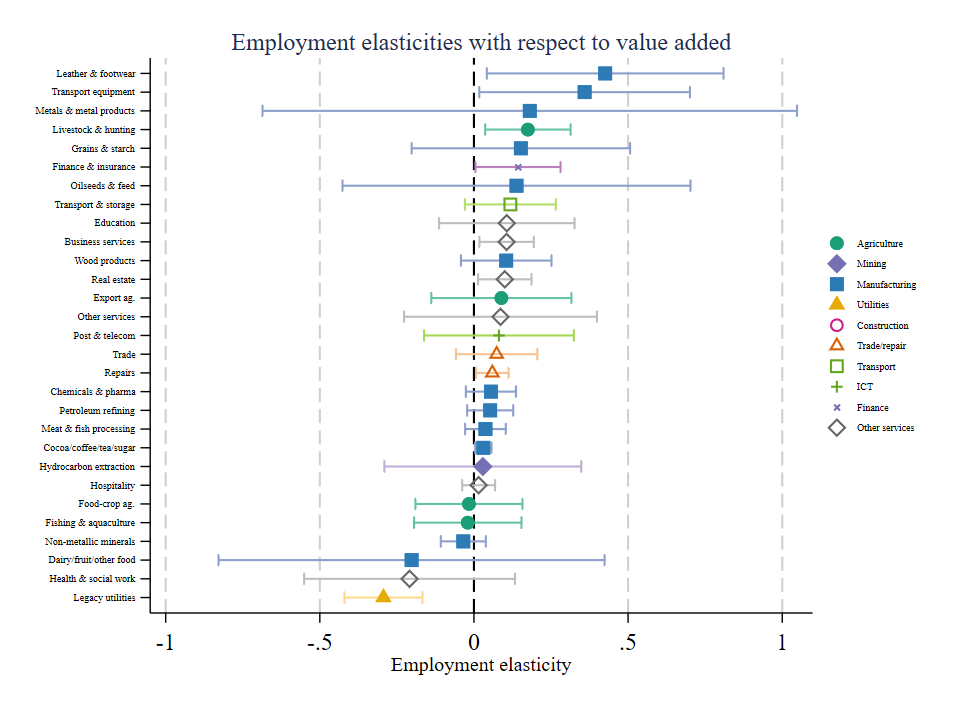
\includegraphics[width=\textwidth,height=0.76\textheight,keepaspectratio]{../output/figures/cmr_nacam_results_en_labels_va_coefficients.png}
\end{frame}

\begin{frame}{Total-Revenue Elasticity Specification}
    \small
    \begin{equation}
        \ln(E_{it}) = \alpha_i + \delta_{st} + \sum_s \beta^{R}_s \left( \ln(R_{it}) \times D_{is} \right) + \varepsilon_{it}
    \end{equation}

    \begin{itemize}
        \item $R_{it}$ is total revenue, estimated in a separate regression from value added.
        \item The sample rule remains at least 30 observations and 10 firms in both reported outcome samples.
        \item The plotted point for each sector is $\beta^{R}_s$ with standard errors clustered at the firm level.
    \end{itemize}
\end{frame}

\begin{frame}{Total-Revenue Elasticities Across NACAM Sectors}
    \centering
    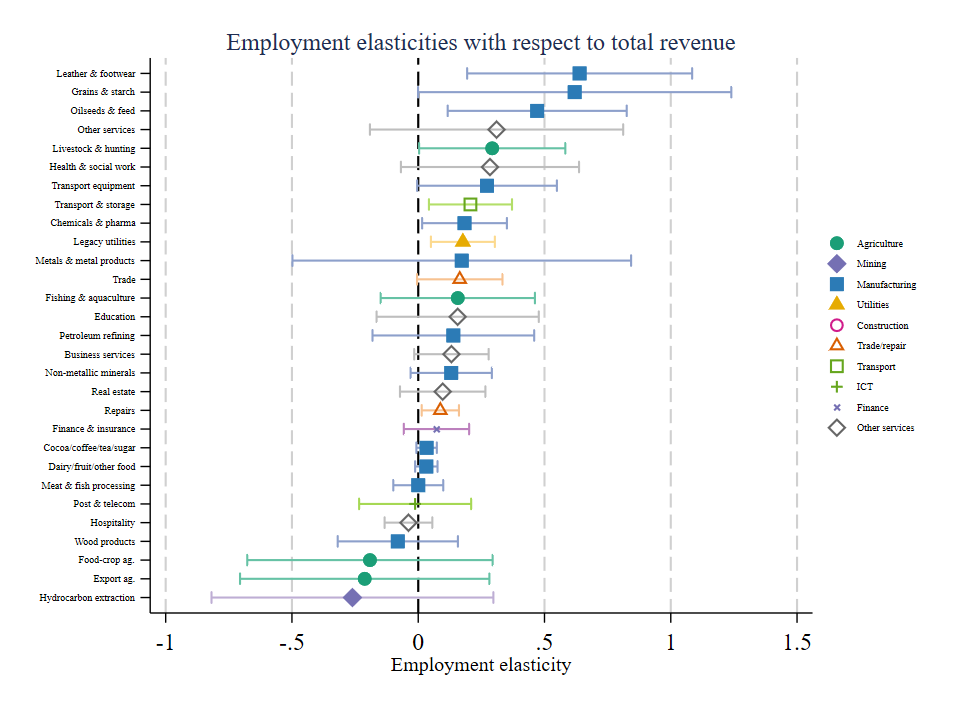
\includegraphics[width=\textwidth,height=0.76\textheight,keepaspectratio]{../output/figures/cmr_nacam_results_en_labels_tot_rev_coefficients.png}
\end{frame}

\begin{frame}{Cross-Model Comparison}
    \begin{itemize}
        \item The next plot compares the sector-specific value-added and total-revenue elasticities.
        \item Each point is one NACAM sector retained by the common inclusion rule.
        \item Points near the 45-degree line indicate sectors where both revenue proxies give similar employment responses.
        \item Large gaps flag sectors where value added and gross revenue tell different stories.
    \end{itemize}
\end{frame}

\begin{frame}{Cross-Model Consistency}
    \centering
    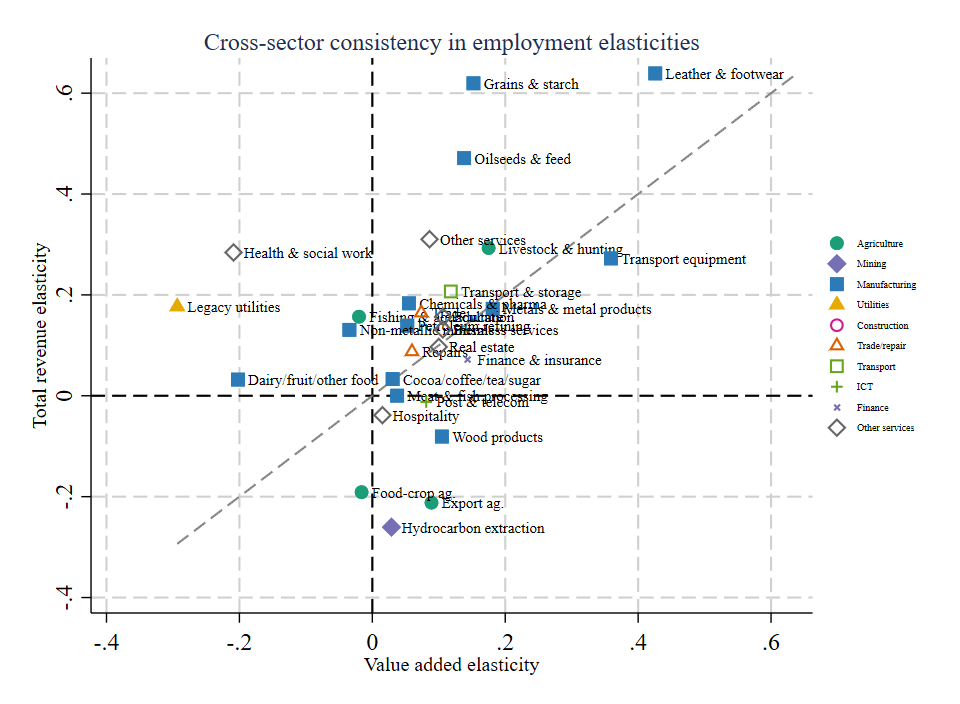
\includegraphics[width=\textwidth,height=0.76\textheight,keepaspectratio]{../output/figures/cmr_nacam_results_en_labels_scatter.png}
\end{frame}

\begin{frame}{Elasticity and Scale Comparison}
    \begin{itemize}
        \item The next scatter plots reuse the same estimated sector elasticities.
        \item Sector scale is calculated from the common valid sample before plotting.
        \item Employment scale uses average firm log employment within sector.
        \item Revenue scale uses average firm log total revenue within sector.
    \end{itemize}
\end{frame}

\begin{frame}{Elasticities and Employment Scale}
    \centering
    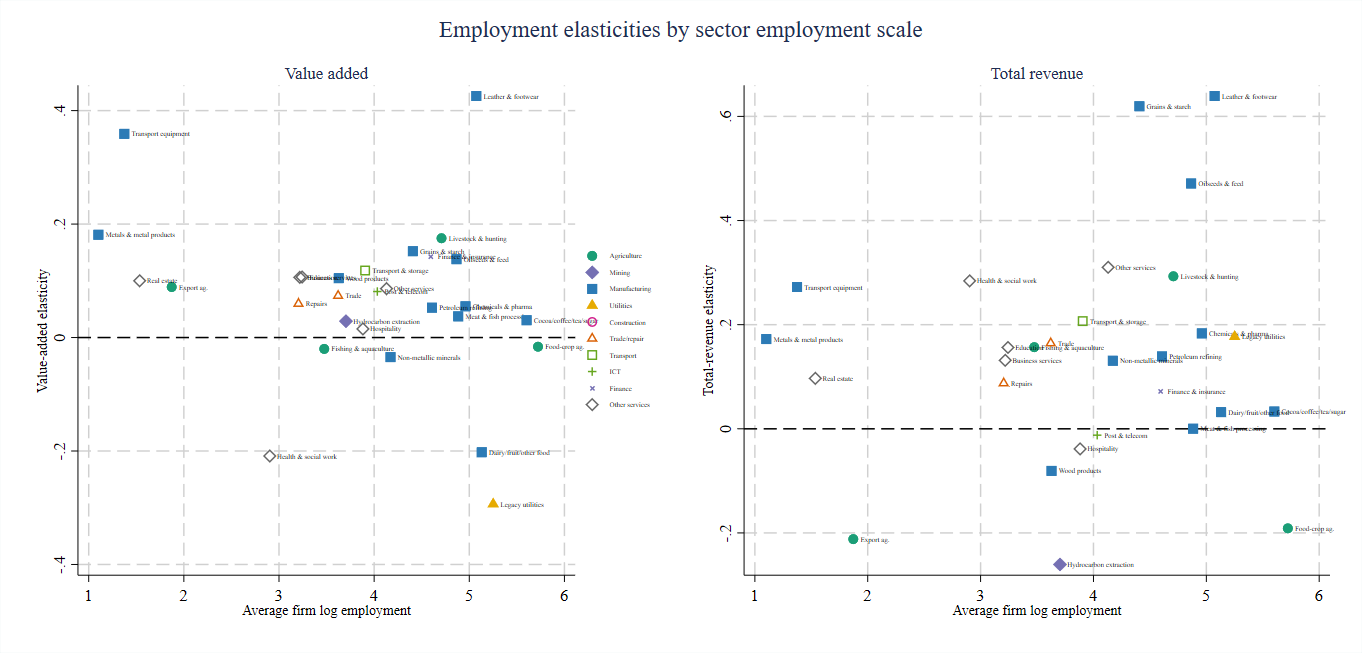
\includegraphics[width=\textwidth,height=0.76\textheight,keepaspectratio]{../output/figures/cmr_nacam_results_en_labels_elasticities_vs_avg_log_employment.png}
\end{frame}

\begin{frame}{Elasticity and Revenue Scale Comparison}
    \begin{itemize}
        \item This plot asks whether high-elasticity sectors are also large-revenue sectors.
        \item Sector labels and included sectors match the administrative elasticity outputs.
    \end{itemize}
\end{frame}

\begin{frame}{Elasticities and Revenue Scale}
    \centering
    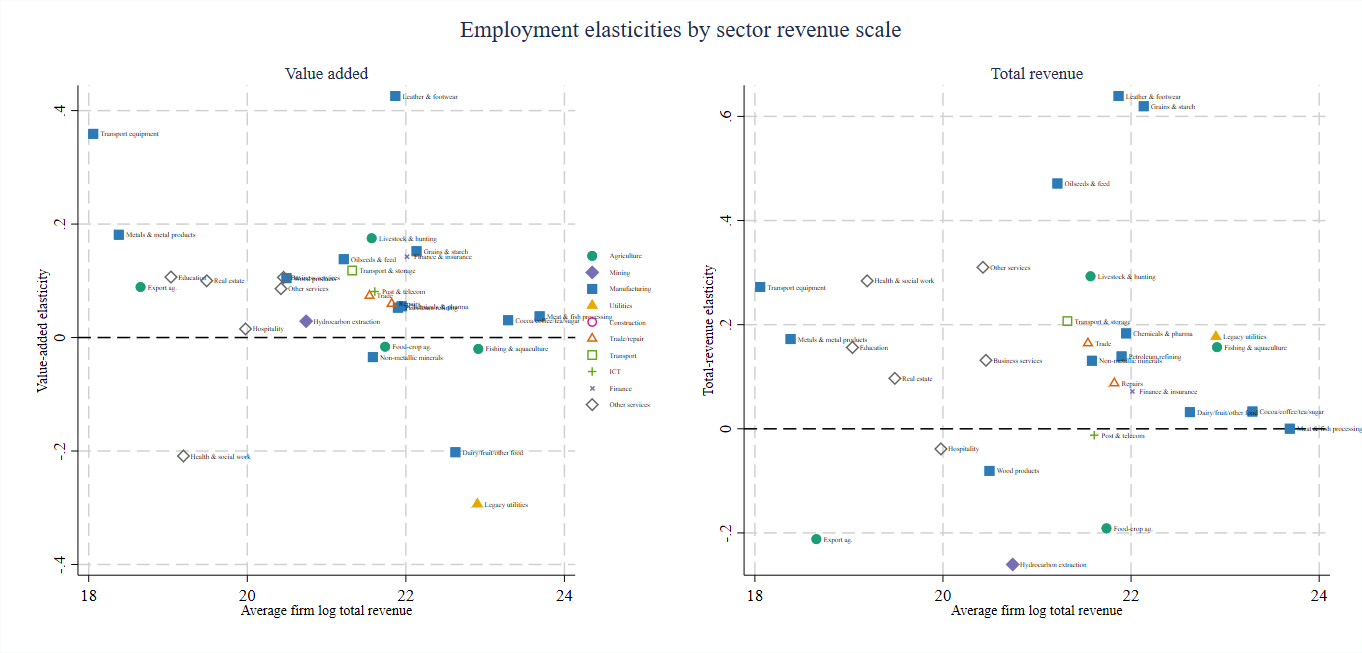
\includegraphics[width=\textwidth,height=0.76\textheight,keepaspectratio]{../output/figures/cmr_nacam_results_en_labels_elasticities_vs_avg_log_revenue.png}
\end{frame}

\begin{frame}{Revenue-Elasticity Sector Deciles}
    \vspace{-0.35cm}
    \centering
    \tiny
    \resizebox{\textwidth}{0.38\textheight}{
        \begin{tabular}{lrrrrr}
                        &Revenue decile&Total revenue elasticity&Value added elasticity&Revenue observations&VA observations\\
\midrule
Leather \& footwear&          10&       0.639&       0.426&         164&         148\\
Grains \& starch&          10&       0.620&       0.152&          78&          67\\
Oilseeds \& feed&           9&       0.471&       0.138&         128&         115\\
Other services&           9&       0.310&       0.086&          60&          55\\
Livestock \& hunting&           9&       0.293&       0.175&         235&         197\\
Health \& social work&           8&       0.284&      -0.209&         263&         243\\
Transport equipment&           8&       0.272&       0.359&         145&         125\\
Transport \& storage&           8&       0.207&       0.118&         788&         708\\
Chemicals \& pharma&           7&       0.183&       0.055&         110&         100\\
Electricity/water supply&           7&       0.177&      -0.294&          56&          54\\
Metals \& metal products&           7&       0.172&       0.181&          53&          45\\
Wholesale/retail&           6&       0.164&       0.074&         654&         575\\
Fishing \& aquaculture&           6&       0.157&      -0.020&          79&          71\\
Education   &           6&       0.156&       0.107&         368&         364\\
Petroleum refining&           5&       0.139&       0.053&         215&         196\\
Services mainly to enterprises&           5&       0.131&       0.106&       1,387&       1,264\\
Non-metallic minerals&           5&       0.131&      -0.035&         222&         183\\
Real estate &           4&       0.097&       0.100&         325&         301\\
Repairs     &           4&       0.088&       0.060&       1,712&       1,522\\
Finance \& insurance&           4&       0.072&       0.143&         300&         272\\
Cocoa/coffee/tea/sugar&           3&       0.033&       0.031&          70&          57\\
Dairy/fruit/other food&           3&       0.032&      -0.202&          76&          64\\
Meat \& fish processing&           3&       0.000&       0.037&          65&          43\\
Post/telecommunications&           2&      -0.012&       0.081&         281&         258\\
Accommodation/food services&           2&      -0.039&       0.015&         241&         224\\
Wood products&           2&      -0.081&       0.105&         183&         171\\
Food crop agriculture&           1&      -0.191&      -0.016&          54&          51\\
Industrial/export agriculture&           1&      -0.212&       0.089&         174&         134\\
Hydrocarbon extraction&           1&      -0.260&       0.029&          59&          48\\

        \end{tabular}
    }
    \vspace{0.03cm}

    {\scriptsize Decile 10 is highest; decile 1 is lowest.}
\end{frame}

\begin{frame}{Main Takeaways}
    \begin{itemize}
        \item Elasticities vary meaningfully across sectors rather than lining up around a single Cameroon-wide coefficient.
        %\item Several sectors show positive employment responses under both value added and total revenue, with NACAM 17 standing out most clearly.
        \item Negative or weak value-added elasticities remain concentrated in a small set of sectors, which is useful for prioritizing follow-up diagnostics.
        %\item The cleaning and harmonization steps are not bookkeeping only; they determine which firm-years and sector codes enter the elasticity analysis.
    \end{itemize}
\end{frame}

\section{CEMAC WBES Trade Analysis}

\begin{frame}{Phase 3: WBES Trade Diagnostics}
    \begin{itemize}
        \item Phase 3 uses the latest available World Bank Enterprise Survey wave for CEMAC countries.
        \item The first step is a cleaning and availability audit for sales, employment, sector, export, import, and input-origin variables.
        \item Gabon is not retained in the main descriptive panels because its latest available WBES wave is 2009 and has no ISIC Rev.4 coverage.
        \item The WBES formal-sector sampling frame covers non-agricultural private firms, so sector rows use eligible activity aggregates rather than agriculture.
    \end{itemize}
\end{frame}

\begin{frame}[plain]
    \centering
    {\small\bfseries WBES Descriptive Statistics}

    \vspace{0.03cm}
    \centering
    \tiny
    \resizebox{0.96\textwidth}{0.46\textheight}{
        \begin{tabular}{lccccccc}
                      &\multicolumn{1}{c}{Cameroon}&\multicolumn{1}{c}{\shortstack{Central Afr.\\Rep.}}&\multicolumn{1}{c}{Chad}&\multicolumn{1}{c}{Congo}&\multicolumn{1}{c}{\shortstack{Eq.\\Guinea}}&\multicolumn{1}{c}{\shortstack{SSA excl.\\CEMAC}}&\multicolumn{1}{c}{\shortstack{High-income\\countries}}\\
\midrule
\textbf{Sample composition}&&&&&&&\\
Fiscal year&2023&2022&2022&2023&2023&2022&2023\\
Surveyed firms&615&151&164&365&173&18252&30855\\
Firms represented (000s)&5&5&1&2&1&354&6879\\
\% Exporting firms&\shortstack{14.6\\{}[2.1]}&\shortstack{28.9\\{}[6.9]}&\shortstack{5.3\\{}[2.5]}&\shortstack{12.9\\{}[2.8]}&\shortstack{15.8\\{}[3.6]}&\shortstack{11.9\\{}[0.6]}&\shortstack{18.8\\{}[0.6]}\\
\% Manufacturing&\shortstack{17.7\\{}[2.7]}&\shortstack{15.2\\{}[5.1]}&\shortstack{28.9\\{}[4.4]}&\shortstack{29.8\\{}[3.6]}&\shortstack{43.3\\{}[4.5]}&\shortstack{24.6\\{}[0.8]}&\shortstack{16.3\\{}[0.5]}\\
\% Construction/utilities&\shortstack{8.8\\{}[1.7]}&\shortstack{15.0\\{}[5.5]}&\shortstack{3.1\\{}[2.3]}&\shortstack{4.0\\{}[1.3]}&\shortstack{7.8\\{}[2.7]}&\shortstack{10.0\\{}[0.7]}&\shortstack{15.1\\{}[0.6]}\\
\% Trade/hospitality/transport&\shortstack{61.7\\{}[3.3]}&\shortstack{67.3\\{}[6.8]}&\shortstack{59.5\\{}[5.3]}&\shortstack{61.4\\{}[3.9]}&\shortstack{34.0\\{}[4.6]}&\shortstack{60.9\\{}[1.0]}&\shortstack{53.3\\{}[0.8]}\\
\% Other services&\shortstack{11.9\\{}[2.0]}&\shortstack{2.5\\{}[1.0]}&\shortstack{8.5\\{}[3.5]}&\shortstack{4.8\\{}[1.9]}&\shortstack{14.8\\{}[3.2]}&\shortstack{4.5\\{}[0.4]}&\shortstack{15.4\\{}[0.7]}\\
\addlinespace \textbf{Economic activity (\% total sales)}&&&&&&&\\
Manufacturing&\shortstack{17.2\\{}[3.2]}&\shortstack{15.6\\{}[5.1]}&\shortstack{16.7\\{}[5.7]}&\shortstack{11.8\\{}[3.9]}&\shortstack{27.6\\{}[6.6]}&\shortstack{31.6\\{}[2.6]}&\shortstack{24.4\\{}[1.2]}\\
Construction/utilities&\shortstack{10.5\\{}[3.3]}&\shortstack{23.0\\{}[11.6]}&\shortstack{3.5\\{}[2.4]}&\shortstack{5.9\\{}[2.8]}&\shortstack{25.8\\{}[9.4]}&\shortstack{16.1\\{}[2.4]}&\shortstack{14.1\\{}[1.4]}\\
Trade/hospitality/transport&\shortstack{59.7\\{}[5.5]}&\shortstack{45.9\\{}[10.0]}&\shortstack{70.1\\{}[7.8]}&\shortstack{78.6\\{}[6.2]}&\shortstack{35.1\\{}[8.9]}&\shortstack{48.8\\{}[2.7]}&\shortstack{45.7\\{}[1.8]}\\
Other services&\shortstack{12.6\\{}[4.4]}&\shortstack{15.4\\{}[10.8]}&\shortstack{9.7\\{}[4.4]}&\shortstack{3.7\\{}[3.4]}&\shortstack{11.5\\{}[6.2]}&\shortstack{3.6\\{}[0.7]}&\shortstack{15.8\\{}[1.5]}\\
\addlinespace \textbf{Average sales (current USD thousands)}&&&&&&&\\
All firms &\shortstack{447.3\\{}[44.3]}&\shortstack{36.0\\{}[6.9]}&\shortstack{312.5\\{}[53.1]}&\shortstack{1058.7\\{}[226.4]}&\shortstack{1075.0\\{}[184.5]}&\shortstack{763.3\\{}[38.3]}&\shortstack{6325.6\\{}[209.6]}\\
Exporting firms&\shortstack{795.4\\{}[166.3]}&\shortstack{47.1\\{}[19.1]}&\shortstack{894.1\\{}[444.0]}&\shortstack{3588.8\\{}[1439.2]}&\shortstack{1002.5\\{}[522.5]}&\shortstack{1771.2\\{}[164.6]}&\shortstack{12779.7\\{}[631.7]}\\
Non-exporting firms&\shortstack{387.4\\{}[43.6]}&\shortstack{31.9\\{}[7.3]}&\shortstack{280.2\\{}[41.5]}&\shortstack{726.7\\{}[164.6]}&\shortstack{1088.0\\{}[197.2]}&\shortstack{633.6\\{}[36.8]}&\shortstack{4801.6\\{}[208.5]}\\
\addlinespace \textbf{Average employment}&&&&&&&\\
All firms &\shortstack{27.8\\{}[2.8]}&\shortstack{22.3\\{}[5.3]}&\shortstack{15.2\\{}[1.6]}&\shortstack{40.9\\{}[9.0]}&\shortstack{32.0\\{}[4.4]}&\shortstack{44.9\\{}[4.9]}&\shortstack{39.2\\{}[4.3]}\\
Exporting firms&\shortstack{51.3\\{}[7.3]}&\shortstack{14.7\\{}[2.9]}&\shortstack{23.0\\{}[6.6]}&\shortstack{151.5\\{}[57.0]}&\shortstack{19.4\\{}[7.4]}&\shortstack{93.5\\{}[19.5]}&\shortstack{73.8\\{}[13.8]}\\
Non-exporting firms&\shortstack{23.8\\{}[3.1]}&\shortstack{24.5\\{}[8.3]}&\shortstack{14.7\\{}[1.7]}&\shortstack{26.4\\{}[4.7]}&\shortstack{34.4\\{}[4.9]}&\shortstack{38.9\\{}[5.1]}&\shortstack{31.1\\{}[4.2]}\\

        \end{tabular}
    }

    \vspace{0.03cm}
    {\tiny Sales use fiscal-year official exchange rates. Brackets report standard errors.}
\end{frame}

\begin{frame}{WBES Country Coverage}
    \footnotesize
    \centering
    \resizebox{0.88\textwidth}{!}{
        \begin{tabular}{lrrrrr}
                        &       Firms&  SurveyYear&  FiscalYear&FirmsWithISIC4&    Retained\\
\midrule
Cameroon    &         615&       2,024&       2,023&         615&           1\\
Central African Republic&         151&       2,023&       2,022&         151&           1\\
Chad        &         164&       2,023&       2,022&         164&           1\\
Congo       &         365&       2,024&       2,023&         365&           1\\
Equatorial Guinea&         173&       2,024&       2,023&         173&           1\\
Gabon       &         179&       2,009&           .&           0&           0\\

        \end{tabular}
    }

    \vspace{0.25cm}
    {\scriptsize Retained excludes Gabon from the main descriptive panels because its latest available wave is 2009 and lacks ISIC Rev.4.}
\end{frame}

\begin{frame}{Core Variable Availability}
    \vspace{-0.2cm}
    \centering
    \tiny
    \resizebox{\textwidth}{!}{
        \begin{tabular}{lrrrrrrrrrrr}
                        &       Firms&       Sales&      SalesW&  Employment&      Weight&       ISIC4& ExportShare&ImportStatus& ImportValue&     FirmAge&OwnershipControls&SalesShareOff100&InputShareOff100&OwnershipShareOff100\\
\midrule
Cameroon    &         615&         614&         614&         615&         615&         615&         615&         613&         275&         614&         614&           0&           0&           0\\
Central African Republic&         151&         139&         139&         151&         151&         151&         134&         126&          56&         147&         128&           0&           0&           0\\
Chad        &         164&         164&         164&         164&         164&         164&         164&         164&         110&         164&         164&           0&           0&           0\\
Congo       &         365&         352&         352&         358&         365&         365&         353&         331&         123&         363&         360&           0&           0&           0\\
Equatorial Guinea&         173&         172&         172&         173&         173&         173&         173&         173&         108&         173&         173&           0&           0&           0\\

        \end{tabular}
    }

    \vspace{0.2cm}
    {\scriptsize Counts are unweighted establishments in retained CEMAC latest-wave surveys.}
\end{frame}

\begin{frame}{Negative Special-Code Audit}
    \vspace{-0.2cm}
    \centering
    \tiny
    \resizebox{\textwidth}{!}{
        \begin{tabular}{lrrrrrrrrrrr}
                        &  Employment&PermanentEmp&       Sales&DomesticShare&IndirectExport&DirectExport&DomesticInput&ForeignInput&DirectImport&  RawMatCost&  ResaleCost\\
\midrule
Cameroon    &           0&           0&           1&           0&           0&           0&           2&           2&           1&          12&           1\\
Central African Republic&           0&           0&          12&          11&          16&          14&          25&          25&          19&           3&           0\\
Chad        &           0&           0&           0&           0&           0&           0&           0&           0&           0&           0&           0\\
Congo       &           0&           7&          13&           6&          10&          10&          34&          34&           1&          27&          42\\
Equatorial Guinea&           0&           0&           1&           0&           0&           0&           0&           0&           0&           0&           0\\

        \end{tabular}
    }

    \vspace{0.2cm}
    {\scriptsize Negative WBES special codes are audited before being recoded to missing for nonnegative levels, percentages, and binary responses.}
\end{frame}

\begin{frame}{Winsorization Cutoffs}
    \footnotesize
    \centering
    \resizebox{0.88\textwidth}{!}{
        \begin{tabular}{lrrrr}
                        &     SalesP5&    SalesP95& InputCostP5&InputCostP95\\
\midrule
Cameroon    &   9,125,300&  2930040000&   2,000,000&  2800000000\\
Central African Republic&   1,744,000& 435,000,000&     300,000&  50,000,000\\
Chad        &   6,750,000&  1115225000&   1,380,000& 500,000,000\\
Congo       &   1,000,000& 12000000000&     150,000& 600,000,000\\
Equatorial Guinea&  13,000,000&  9090000000&     300,000& 669,000,000\\

        \end{tabular}
    }

    \vspace{0.25cm}
    {\scriptsize Sales and input costs are winsorized at the 5th and 95th percentiles within each country wave.}
\end{frame}

\begin{frame}{Exporter Participation}
    \centering
    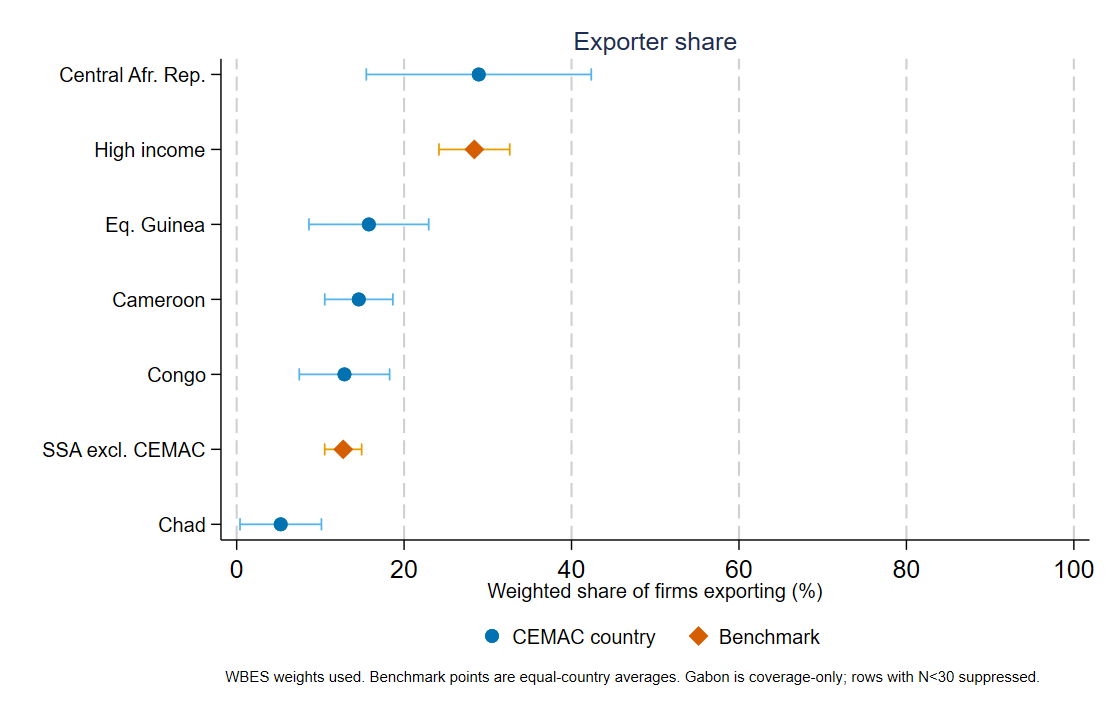
\includegraphics[width=\textwidth,height=0.78\textheight,keepaspectratio]{../output/figures/cemac_wbes_trade_exporter_share.png}
\end{frame}

\begin{frame}{Export Intensity Among Exporters}
    \centering
    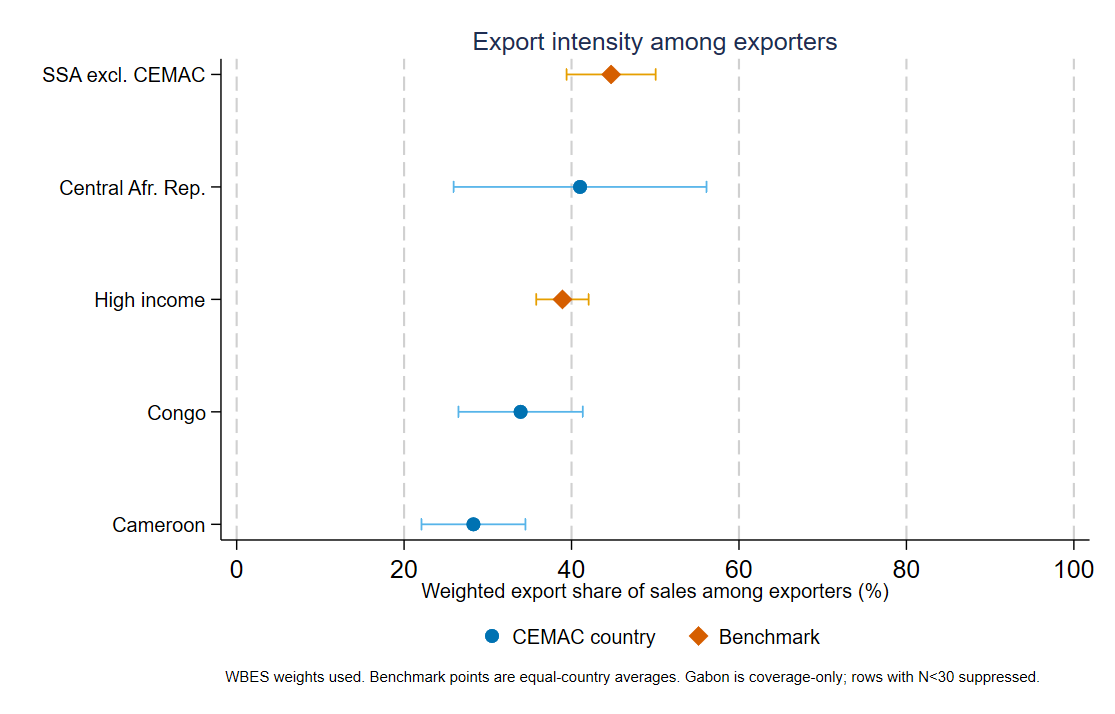
\includegraphics[width=\textwidth,height=0.78\textheight,keepaspectratio]{../output/figures/cemac_wbes_trade_export_intensity.png}
\end{frame}

\begin{frame}{Import and Foreign-Input Participation}
    \centering
    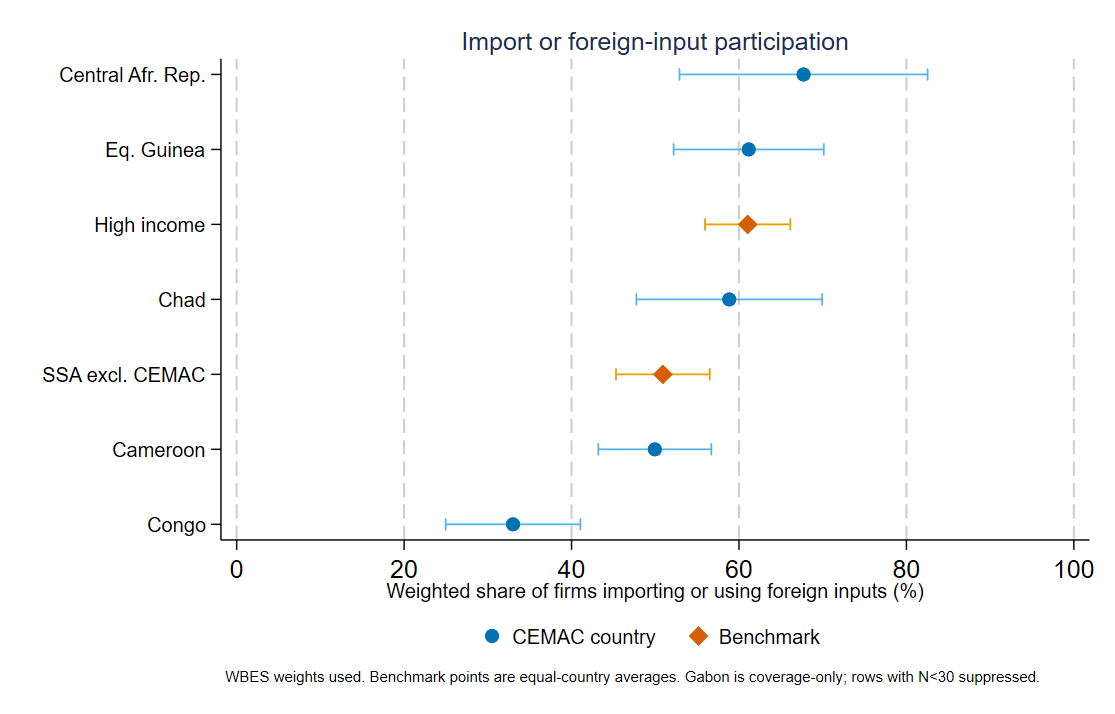
\includegraphics[width=\textwidth,height=0.78\textheight,keepaspectratio]{../output/figures/cemac_wbes_trade_import_participation.png}
\end{frame}

\begin{frame}{Two-Way Trader Status}
    \centering
    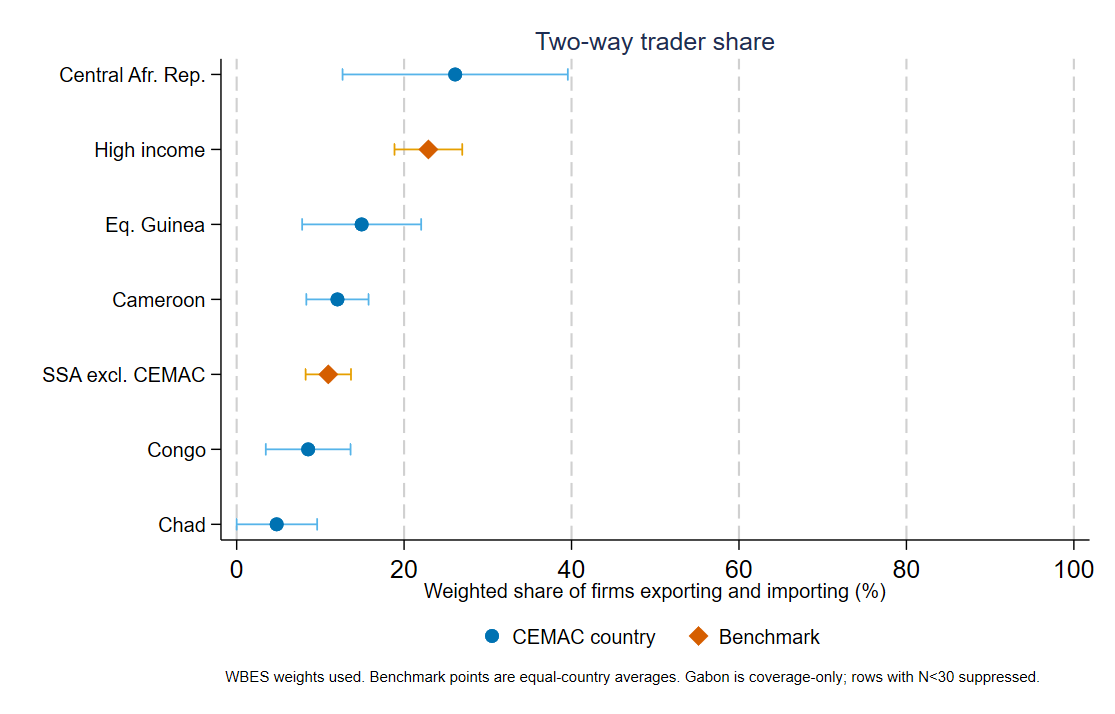
\includegraphics[width=\textwidth,height=0.78\textheight,keepaspectratio]{../output/figures/cemac_wbes_trade_two_way_trader.png}
\end{frame}

\begin{frame}{WBES Trade-Employment Association}
    \small
    \begin{equation}
        \ln(E_i) = \alpha + \beta \ln(X_i^+) + \gamma Exporter_i + \varepsilon_i
    \end{equation}

    \begin{itemize}
        \item Latest-wave WBES estimates are weighted cross-sectional associations.
        \item $X_i^+$ is export value, with log export value set to zero for non-exporters in the all-firm model.
        \item The exporter dummy separates the extensive margin from the positive-export-value slope.
        \item Rows with fewer than 30 observations are suppressed; benchmark rows are equal-country averages.
    \end{itemize}
\end{frame}

\begin{frame}{WBES Country Trade-Employment Estimates}
    \vspace{-0.2cm}
    \centering
    \tiny
    \resizebox{\textwidth}{!}{
        \begin{tabular}{lrrrrrrrr}
                        &All-firm slope&          SE&           N&   Exporters&Exporter-only slope&          SE&           N&   Countries\\
\midrule
Cameroon    &       0.325&       0.038&         613&         136&       0.373&       0.040&         136&           1\\
Central Afr. Rep.&      -0.117&       0.208&         112&          36&      -0.273&       0.113&          36&           1\\
Chad        &      -0.044&       0.176&         164&          13&           .&           .&           .&           1\\
Congo       &       0.115&       0.045&         340&          46&       0.118&       0.068&          46&           1\\
Eq. Guinea  &       0.297&       0.118&         172&          18&           .&           .&           .&           1\\
CEMAC average&       0.115&       0.088&       1,401&         249&       0.072&       0.188&         218&           5\\
High income &       0.299&       0.014&      29,863&      10,704&       0.319&       0.013&      10,642&          45\\
SSA excl. CEMAC&       0.240&       0.031&      16,820&       2,724&       0.269&       0.027&       2,546&          38\\

        \end{tabular}
    }

    \vspace{0.15cm}
    {\scriptsize Slopes are weighted cross-sectional log employment/log export-value associations.}
\end{frame}

\begin{frame}{WBES Country Specification: All Firms}
    \small
    \begin{equation}
        \ln(E_i) = \alpha_c + \beta_c \ln(X_i^+) + \gamma_c Exporter_i + \varepsilon_i
    \end{equation}

    \begin{itemize}
        \item Estimated separately by country using WBES weights.
        \item Non-exporters stay in the sample with $\ln(X_i^+) = 0$.
        \item The plotted coefficient is $\beta_c$; it is descriptive, not causal.
    \end{itemize}
\end{frame}

\begin{frame}{WBES Country Associations: All Firms}
    \centering
    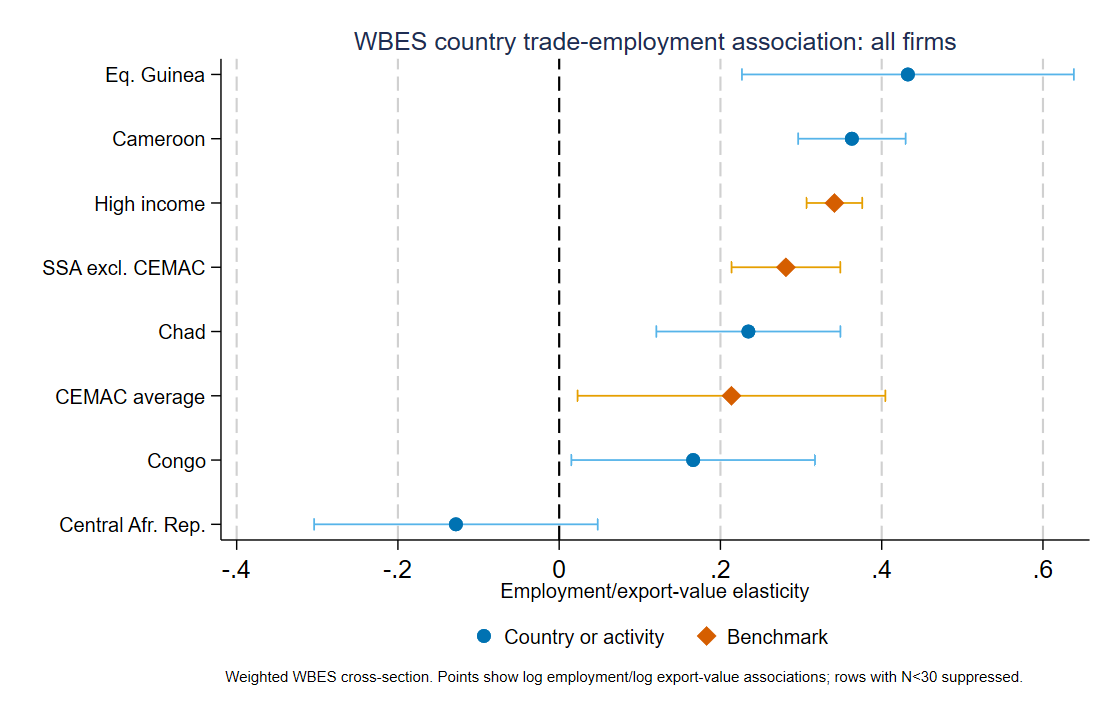
\includegraphics[width=\textwidth,height=0.78\textheight,keepaspectratio]{../output/figures/cemac_wbes_trade_elasticity_country_all_firms.png}
\end{frame}

\begin{frame}{WBES Country Specification: Exporters Only}
    \small
    \begin{equation}
        \ln(E_i) = \alpha_c + \beta_c \ln(X_i) + \varepsilon_i,\quad X_i > 0
    \end{equation}

    \begin{itemize}
        \item Estimated separately by country among firms with positive export value.
        \item This is the intensive-margin association within exporters.
        \item Countries with fewer than 30 exporters are suppressed in the plot.
    \end{itemize}
\end{frame}

\begin{frame}{WBES Country Associations: Exporters Only}
    \centering
    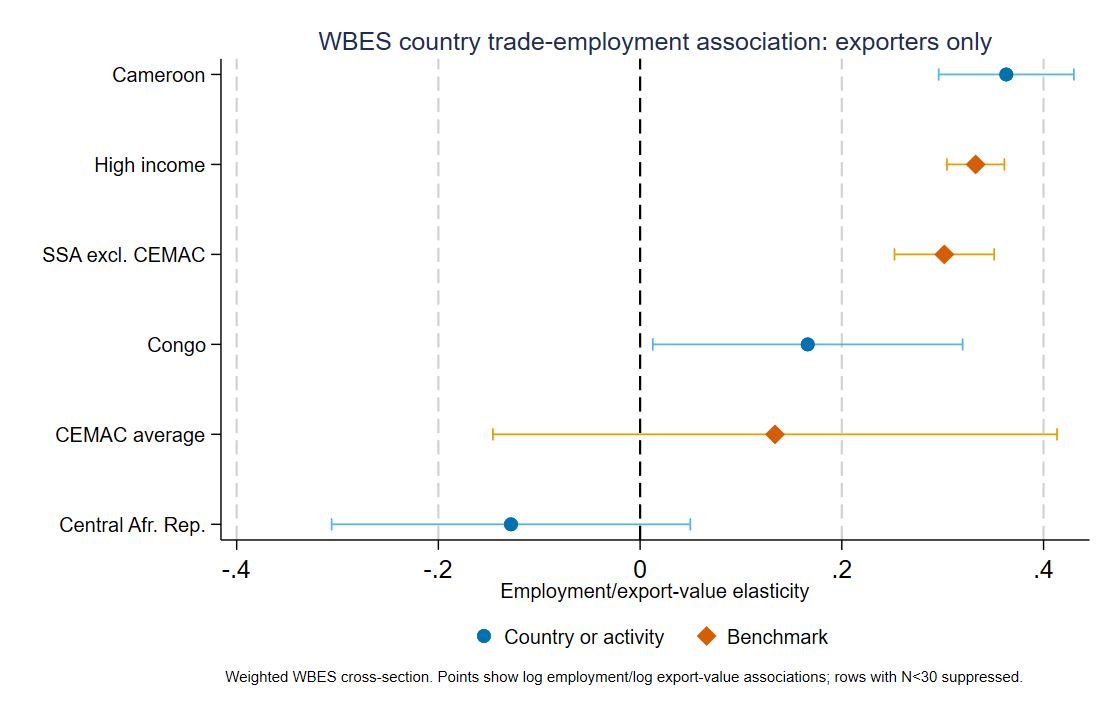
\includegraphics[width=\textwidth,height=0.78\textheight,keepaspectratio]{../output/figures/cemac_wbes_trade_elasticity_country_exporters_only.png}
\end{frame}

\begin{frame}{Cameroon WBES Activity Estimates}
    \vspace{-0.2cm}
    \centering
    \tiny
    \resizebox{0.96\textwidth}{!}{
        \begin{tabular}{lrrrrrrr}
                        &All-firm slope&          SE&           N&   Exporters&Exporter-only slope&          SE&           N\\
\midrule
Construction/utilities&       0.216&       0.201&          60&           8&           .&           .&           .\\
Manufacturing&       0.546&       0.064&         161&          53&       0.546&       0.065&          53\\
Other services&       0.373&       0.037&          52&           9&           .&           .&           .\\
Trade/hospitality/transport&       0.300&       0.049&         342&          68&       0.300&       0.050&          68\\

        \end{tabular}
    }

    \vspace{0.15cm}
    {\scriptsize Activity groups use WBES-ISIC aggregates}
\end{frame}

\begin{frame}{Cameroon Activity Specification: All Firms}
    \small
    \begin{equation}
        \ln(E_i) = \alpha_a + \beta_a \ln(X_i^+) + \gamma_a Exporter_i + \varepsilon_i
    \end{equation}

    \begin{itemize}
        \item Estimated within Cameroon WBES activity groups.
        \item This is a diagnostic adaptation of the elasticity idea to cross-sectional survey data.
        \item Activity rows pass the all-firm sample threshold, but exporter-only rows may be suppressed.
    \end{itemize}
\end{frame}

\begin{frame}{Cameroon Activity Associations: All Firms}
    \centering
    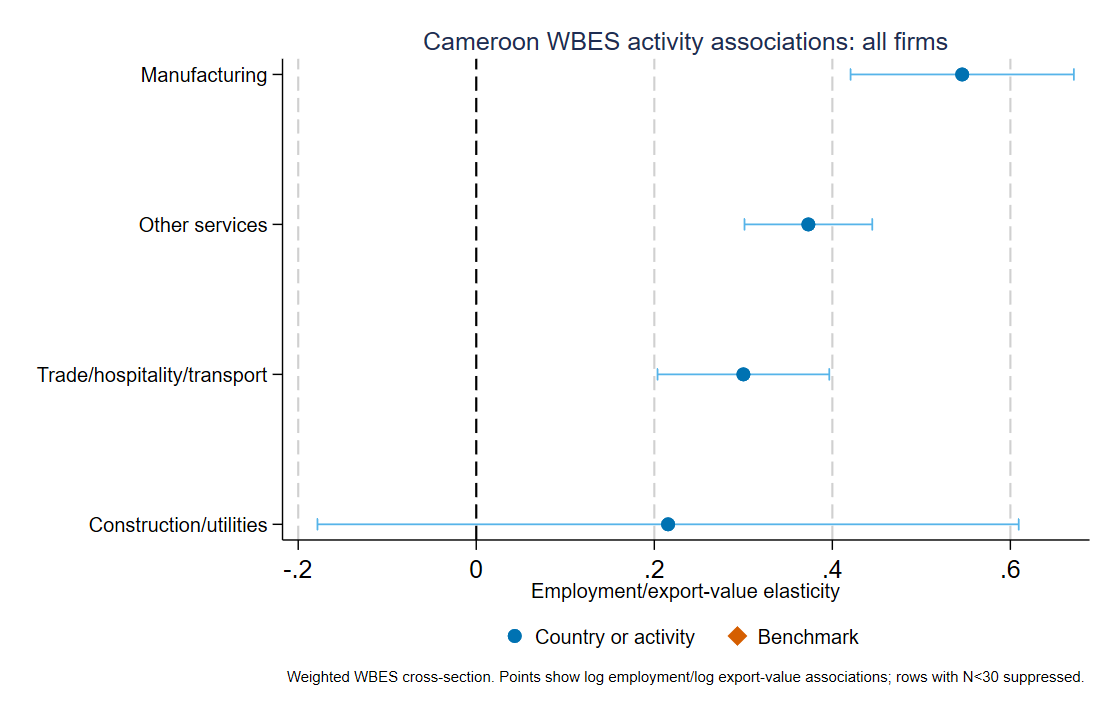
\includegraphics[width=\textwidth,height=0.78\textheight,keepaspectratio]{../output/figures/cemac_wbes_trade_elasticity_cameroon_activity_all_firms.png}
\end{frame}

\begin{frame}{Cameroon Activity Specification: Exporters Only}
    \small
    \begin{equation}
        \ln(E_i) = \alpha_a + \beta_a \ln(X_i) + \varepsilon_i,\quad X_i > 0
    \end{equation}

    \begin{itemize}
        \item Estimated among Cameroon exporters within WBES activity groups.
        \item Rows are shown only when at least 30 exporter observations are available.
        \item These results are best read as sample diagnostics for follow-up, not sector multipliers.
    \end{itemize}
\end{frame}

\begin{frame}{Cameroon Activity Associations: Exporters Only}
    \centering
    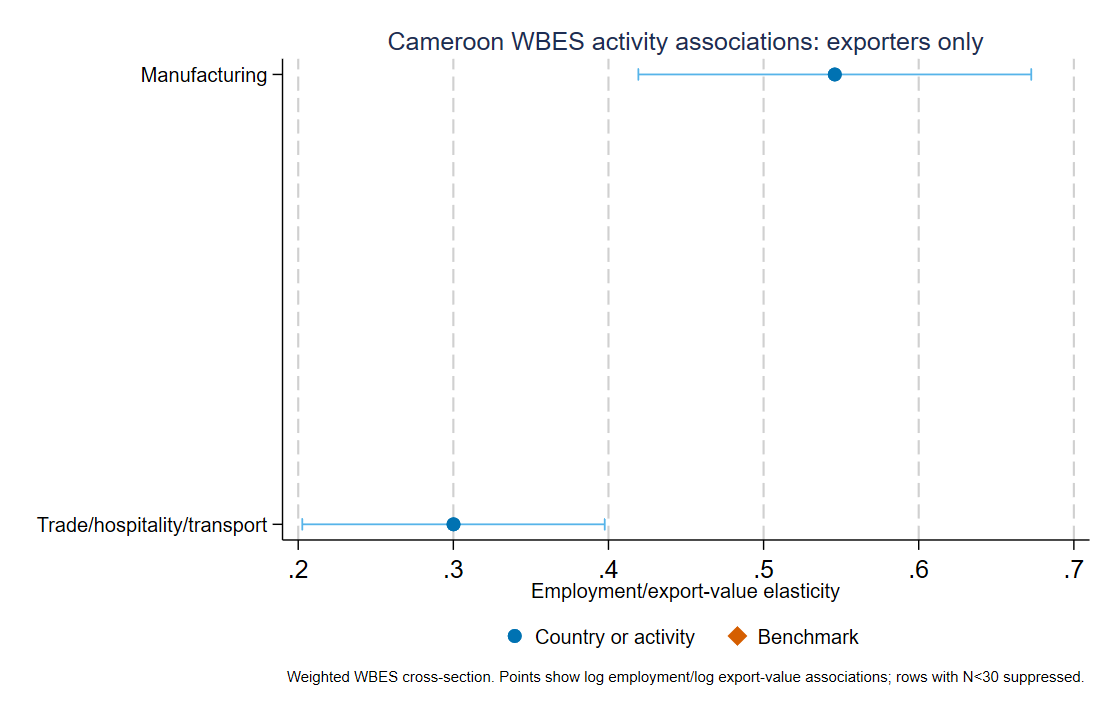
\includegraphics[width=\textwidth,height=0.78\textheight,keepaspectratio]{../output/figures/cemac_wbes_trade_elasticity_cameroon_activity_exporters_only.png}
\end{frame}

\end{document}
